% Présentation courte : modèle réduit à encodeur-décodeur linéaire (partie 2, étape 1)
% Compilation : cd presentation && pdflatex reduction_lineaire.tex && pdflatex reduction_lineaire.tex
% Figures : python3 presentation/figures.py (après main.py et main_reduction.py)
\documentclass[aspectratio=169, 11pt]{beamer}
\usetheme[progressbar=frametitle, numbering=fraction, sectionpage=none]{metropolis}
\usepackage[T1]{fontenc}
\usepackage{lmodern}
\usepackage{amsmath, amssymb, mathtools}
\usepackage{booktabs}
\usepackage{tikz}
\usetikzlibrary{arrows.meta, positioning}
\graphicspath{{figures/}}

\definecolor{bleu}{HTML}{1F4E79}
\definecolor{rouge}{HTML}{B22222}
\setbeamercolor{alerted text}{fg=rouge}

\newcommand{\R}{\mathbb{R}}
\newcommand{\ubar}{\bar u}
\newcommand{\Ah}{\hat A}
\newcommand{\ch}{\hat c}
\newcommand{\cit}[1]{{\footnotesize\textcolor{gray}{[#1]}}}   % citation dans le texte

\title{Encodeur-décodeur linéaire pour la chaleur 1D à données aléatoires}
\subtitle{Partie 2, étape 1 : la référence avant les encodeurs non linéaires}
\author{Anass Aboufadel}
\date{Novembre 2026}

\begin{document}

\maketitle

% -----------------------------------------------------------------------------------------------------
\begin{frame}{Problème et objectif}
  \vspace{-0.6em}
  \[
    \partial_t u = \partial_x(k\,\partial_x u) + f, \ \ u(0) = u(1) = 0, \ \ u(x,0) = \sin(\pi x)
    \ \ \Longrightarrow\ \ \dot u = A(\nu)\,u + b(\nu)
  \]
  {\small Deux cas séparés, $M = 3$ zones : conductivité $k_m \sim \mathrm{LogN}(0, 0.3^2)$ avec $f = 1$, \emph{ou}
  source $s_m \sim \mathcal U(0.5, 1.5)$ avec $k = 1$. Partie 1 : Monte Carlo, 500 tirages.}

  \vspace{0.2em}
  \centering
  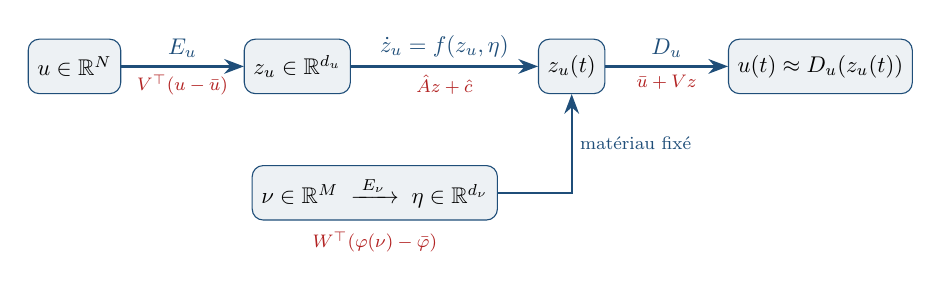
\begin{tikzpicture}[scale=0.82, transform shape,
      boite/.style={draw=bleu, rounded corners, fill=bleu!8, minimum height=2.4em, inner sep=4pt},
      fl/.style={-{Stealth[length=2.5mm]}, thick, bleu}, lab/.style={font=\footnotesize, text=rouge}]
    \node[boite] (u) {$u \in \R^N$};
    \node[boite, right=1.9cm of u] (z) {$z_u \in \R^{d_u}$};
    \node[boite, right=2.9cm of z] (zt) {$z_u(t)$};
    \node[boite, right=1.9cm of zt] (ut) {$u(t) \approx D_u(z_u(t))$};
    \node[boite, below=1.1cm of z, xshift=1.2cm] (nu) {$\nu \in \R^M \;\xrightarrow{\;E_\nu\;}\; \eta \in \R^{d_\nu}$};
    \draw[fl] (u) -- node[above]{$E_u$} node[below, lab]{$V^\top(u - \ubar)$} (z);
    \draw[fl] (z) -- node[above]{$\dot z_u = f(z_u, \eta)$} node[below, lab]{$\Ah z + \ch$} (zt);
    \draw[fl] (zt) -- node[above]{$D_u$} node[below, lab]{$\ubar + V z$} (ut);
    \draw[fl] (nu.east) -| node[pos=0.75, right, font=\footnotesize]{matériau fixé} (zt.south);
    \node[lab, below=0.05cm of nu] {$W^\top(\varphi(\nu) - \bar\varphi)$};
  \end{tikzpicture}

  \raggedright
  {\small Réduire $u$ \emph{et} $\nu$ pour transporter la loi par Liouville avec $d_u = d_\nu = 2$ \cit{Iollo}.
  Ici, la version \alert{entièrement linéaire} (en rouge).}
\end{frame}

% -----------------------------------------------------------------------------------------------------
\begin{frame}{Pourquoi commencer par le linéaire ?}
  \begin{columns}[T]
    \begin{column}{0.54\textwidth}
      \begin{itemize}\small
        \item \textbf{Diffusif} : $A(\nu)$ symétrique définie négative, le mode $j$ est amorti en $e^{-j^2\pi^2 t}$ ;
          solution régulière pour $t > 0$.
        \item \textbf{Pas de transport} : rien ne se déplace ; les coudes (conductivité) restent aux interfaces fixes
          $x = 1/3,\ 2/3$.
        \item \textbf{Régulier en $\nu$} : $u^*$ affine en $s$, rationnelle donc holomorphe en $k$
          $\Rightarrow$ $n$-épaisseurs de Kolmogorov à décroissance exponentielle \cit{Cohen \& DeVore, 2015}.
        \item \textbf{Linéaire en $u$, affine en $\nu$} : Galerkin donne exactement $\dot z = \Ah z + \ch$.
      \end{itemize}
    \end{column}
    \begin{column}{0.44\textwidth}
      \centering
      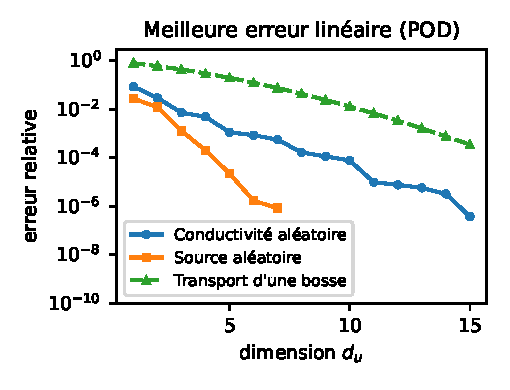
\includegraphics[width=\textwidth]{spectre_erreur}
      {\footnotesize Transport : $\approx 10$ modes pour $10^{-2}$, d'où les décodeurs non linéaires
      \cit{Lee \& Carlberg, 2020}. Ici, 3 modes suffisent.}
    \end{column}
  \end{columns}
\end{frame}

% -----------------------------------------------------------------------------------------------------
\begin{frame}{État et dynamique latente}
  \begin{columns}[T]
    \begin{column}{0.47\textwidth}
      \textbf{État : POD} {\small (400 matériaux $\times$ 51 instants)}
      \[ E_u(u) = V^\top(u - \ubar), \qquad D_u(z) = \ubar + V z \]
      \begin{itemize}\small
        \item Optimal parmi les encodeurs-décodeurs linéaires \cit{Eckart \& Young, 1936}.
        \item C'est ce qu'apprend un autoencodeur linéaire \cit{Baldi \& Hornik, 1989}.
        \item $u_0$ fixé : $z_0 = E_u(u_0)$ est commun à tous les matériaux.
      \end{itemize}
    \end{column}
    \begin{column}{0.51\textwidth}
      \textbf{Dynamique : Galerkin} \cit{Benner et al., 2015}
      \begin{gather*}
        \dot z = \Ah(\eta)\,z + \ch(\eta) \\
        \Ah = V^\top A V, \qquad \ch = V^\top(A\ubar + b)
      \end{gather*}
      {\small $(A, b)$ assemblés pour le matériau $\tilde\nu = D_\nu(\eta)$.}
      \begin{itemize}\small
        \item $\Ah$ symétrique définie négative : \alert{stable}, équilibre unique $z^*(\eta) = -\Ah^{-1}\ch$.
        \item Intégration exacte : $z(t) = z^* + Q e^{\Lambda t} Q^\top (z_0 - z^*)$.
        \item $\nabla_z \cdot f = \operatorname{tr}\Ah$ constant : test exact pour la Liouville (partie 3).
      \end{itemize}
    \end{column}
  \end{columns}
\end{frame}

% -----------------------------------------------------------------------------------------------------
\begin{frame}{Matériau : sous-espace actif plutôt qu'ACP}
  \begin{columns}[T]
    \begin{column}{0.57\textwidth}
      \begin{itemize}\small
        \item Les $\nu_m$ sont i.i.d. : covariance isotrope, une ACP de $\nu$ ne réduit rien.
        \item On garde les directions qui \textbf{changent la solution} \cit{Constantine, 2015} :
          \[ C = \mathbb E[J^\top J], \quad J = \frac{\partial u^*}{\partial \varphi}, \quad
             \eta = W^\top(\varphi(\nu) - \bar\varphi), \]
          avec $\varphi = \log k$ ou $\varphi = s$.
        \item Conductivité : $\eta_1 \approx k_1 + k_3$, $\eta_2 \approx k_1 - k_3$ ; $k_2$ pèse peu car le flux est
          \alert{nul au centre}.
        \item Source : $s_2$ domine (fonction de Green maximale au centre), puis $s_3 - s_1$.
        \item $d_\nu = 2$ garde $\approx 99\,\%$ de la sensibilité.
      \end{itemize}
    \end{column}
    \begin{column}{0.41\textwidth}
      \centering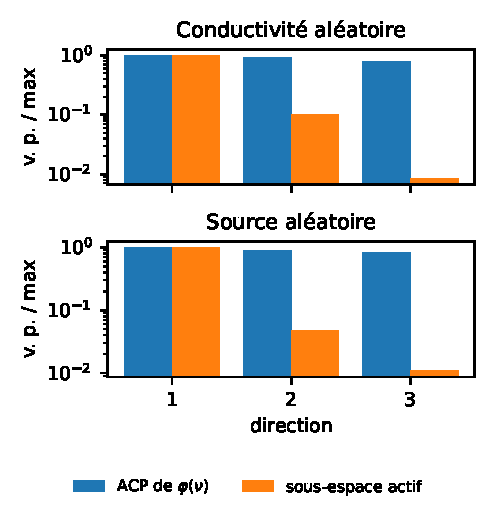
\includegraphics[height=0.74\textheight]{materiau}
    \end{column}
  \end{columns}
\end{frame}

% -----------------------------------------------------------------------------------------------------
\begin{frame}{Validation : tests élémentaires}
  \begin{columns}[c]
    \begin{column}{0.55\textwidth}
      \footnotesize\setlength{\tabcolsep}{4pt}
      \begin{tabular}{lr}
        \toprule
        Test (deux cas, 2.6 s) & Écart \\
        \midrule
        Base orthonormée, $E_u \circ D_u = \mathrm{id}$ & $10^{-15}$ \\
        Erreur de projection $= \sum_{j > d} \sigma_j^2$ & $2\cdot 10^{-14}$ \\
        Équilibres source de rang 3 & $3\cdot 10^{-16}$ \\
        Gradient différences finies / analytique & $7\cdot 10^{-10}$ \\
        $d_u = N$, $d_\nu = M$ : réduit = complet & $10^{-9}$ \\
        Intégration exacte / $\exp(\Ah t)$ & $2\cdot 10^{-15}$ \\
        $\lambda_{\max}(\Ah)$, $d_u = 2$ & $-6.7$ / $-9.87$ \\
        \bottomrule
      \end{tabular}
    \end{column}
    \begin{column}{0.43\textwidth}
      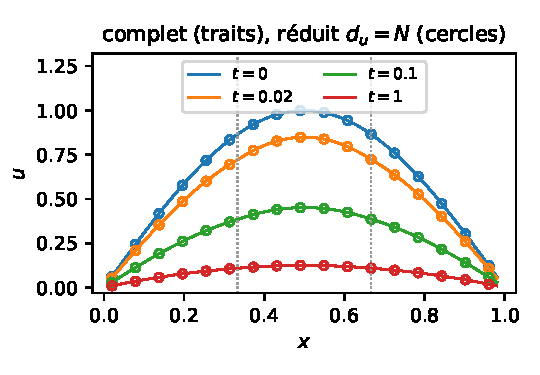
\includegraphics[width=\textwidth]{validation}
      {\footnotesize Avec toute la base, le réduit redonne le complet ($10^{-9}$ = tolérance du BDF).}
    \end{column}
  \end{columns}
\end{frame}

% -----------------------------------------------------------------------------------------------------
\begin{frame}{Erreur sur 100 matériaux non vus}
  \centering
  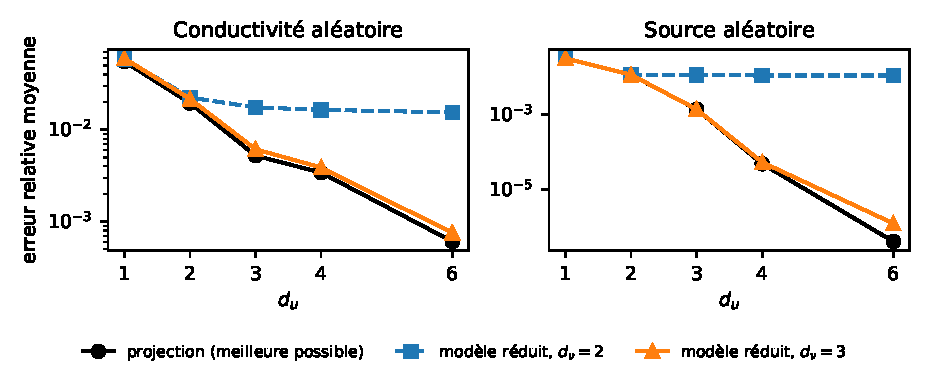
\includegraphics[height=0.55\textheight]{erreurs}
  \begin{itemize}\small
    \item $d_\nu = 3$ : réduit $\approx$ projection $\Rightarrow$ \alert{fermeture vérifiée}, les variables latentes
      suffisent à prédire.
    \item $d_\nu = 2$ : plateau ($\approx 1.5\,\%$ et $1.1\,\%$) : c'est la réduction du matériau qui limite.
    \item $d_u = d_\nu = 2$ : $2.2\,\%$ (conductivité) et $1.2\,\%$ (source) en moyenne ; max $22\,\%$ pour les
      matériaux très contrastés.
  \end{itemize}
\end{frame}

% -----------------------------------------------------------------------------------------------------
\begin{frame}{Plan latent et propagation de l'incertitude ($d_u = d_\nu = 2$)}
  \centering
  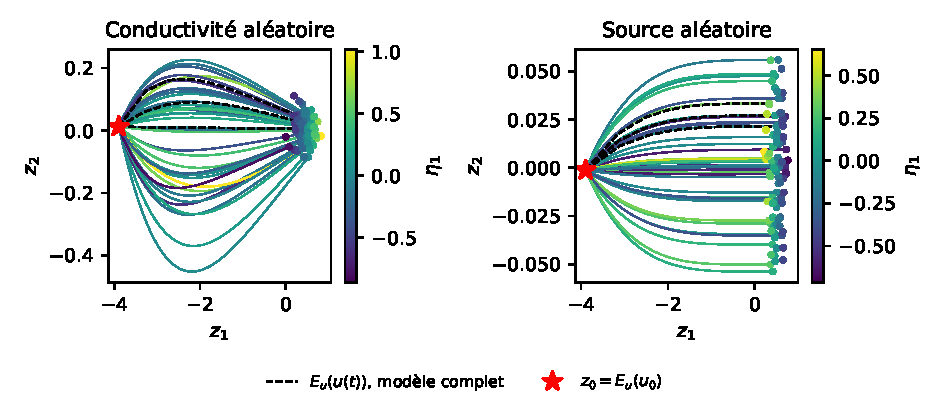
\includegraphics[height=0.56\textheight]{plan_latent}
  \begin{itemize}\small
    \item Toutes les trajectoires partent de $z_0$ et rejoignent $z^*(\eta)$ : c'est le plan de la Liouville
      (partie 3).
    \item Face au Monte Carlo (500 matériaux) : $E[T^*]$ passe de $0.0874$ à $0.0870$ et de $0.0868$ à $0.0868$,
      écarts dans l'IC à 95\,\% ; coût par matériau divisé par $\approx 75$.
  \end{itemize}
\end{frame}

% -----------------------------------------------------------------------------------------------------
\begin{frame}{Bilan et suite}
  \textbf{Bilan}
  \begin{itemize}\small
    \item Problème diffusif et régulier : le linéaire est quasi optimal et sert de référence.
    \item Hypothèse essentielle vérifiée dans le cas linéaire ; statistiques de $T$ dans l'IC du Monte Carlo.
    \item Limites : $d_\nu = 2$ et matériaux très contrastés.
  \end{itemize}
  \textbf{Suite}
  \begin{enumerate}\small
    \item Autoencodeur convolutif 1D \cit{Lee \& Carlberg, 2020}, de type U-Net \cit{Ronneberger et al., 2015} mais
      \emph{sans} sauts depuis l'état, qui contourneraient le goulot \cit{Falck et al., 2022}.
      Cible : battre $2.2\,\% / 22\,\%$ à $d_u = 2$.
    \item Encodeur du matériau non linéaire, appris avec la dynamique (pertes sur les dérivées latentes
      \cit{Champion et al., 2019}).
    \item Liouville réduite par volumes finis dans le plan $(z_1, z_2)$ \cit{Iollo}.
  \end{enumerate}
\end{frame}

% -----------------------------------------------------------------------------------------------------
\begin{frame}{Références}
  \scriptsize\setlength{\parskip}{4pt}
  \begin{columns}[T]
    \begin{column}{0.49\textwidth}\raggedright
      \textcolor{gray}{[Baldi \& Hornik, 1989]} P. Baldi, K. Hornik, Neural networks and principal component analysis: learning from examples without local minima, \emph{Neural Networks} 2(1):53--58.\par
      \textcolor{gray}{[Benner et al., 2015]} P. Benner, S. Gugercin, K. Willcox, A survey of projection-based model reduction methods for parametric dynamical systems, \emph{SIAM Review} 57(4):483--531.\par
      \textcolor{gray}{[Champion et al., 2019]} K. Champion, B. Lusch, J. N. Kutz, S. L. Brunton, Data-driven discovery of coordinates and governing equations, \emph{PNAS} 116(45):22445--22451.\par
      \textcolor{gray}{[Cohen \& DeVore, 2015]} A. Cohen, R. DeVore, Approximation of high-dimensional parametric PDEs, \emph{Acta Numerica} 24:1--159.\par
      \textcolor{gray}{[Constantine, 2015]} P. G. Constantine, \emph{Active Subspaces: Emerging Ideas for Dimension Reduction in Parameter Studies}, SIAM.\par
    \end{column}
    \begin{column}{0.49\textwidth}\raggedright
      \textcolor{gray}{[Eckart \& Young, 1936]} C. Eckart, G. Young, The approximation of one matrix by another of lower rank, \emph{Psychometrika} 1(3):211--218.\par
      \textcolor{gray}{[Falck et al., 2022]} F. Falck et al., A multi-resolution framework for U-Nets with applications to hierarchical VAEs, \emph{NeurIPS}.\par
      \textcolor{gray}{[Iollo]} A. Iollo, \emph{Réduction d'incertitude par l'équation de Liouville}, support de cours.\par
      \textcolor{gray}{[Lee \& Carlberg, 2020]} K. Lee, K. Carlberg, Model reduction of dynamical systems on nonlinear manifolds using deep convolutional autoencoders, \emph{J. Comput. Phys.} 404:108973.\par
      \textcolor{gray}{[Ronneberger et al., 2015]} O. Ronneberger, P. Fischer, T. Brox, U-Net: convolutional networks for biomedical image segmentation, \emph{MICCAI}.\par
    \end{column}
  \end{columns}
\end{frame}

\end{document}
